\documentclass[../labs.tex]{subfiles}
\begin{document}

\chapter{Exercise 1: A simple neural network}
\label{ch:lab01_ex1}

This exercise introduces the computational path shared by larger learning systems: represent data as tensors, define a parameterized model, measure prediction error, and update the parameters from gradients. Its final objective is to fit a univariate linear relation in PyTorch and recover the known generating rule from synthetic observations. Inputs are scalar features paired with noisy targets; the expected result is a trained weight and bias close to the values used to produce those targets. We begin with tensor operations and precision because the same data representation supports the model and its optimizer.

\section{Tensor operations, precision, and device selection}

PyTorch tensors extend array operations with device placement and automatic differentiation. The opening cells import the runtime, confirm basic elementwise arithmetic and dtype behavior, and benchmark matrix multiplication in float64 and float32. The benchmark is an observation from this execution environment: its result depends on the selected device, warm-up, system load, and library implementation. Device selection later keeps the model and its inputs on the same processor.


\noindent This setup cell imports the libraries used throughout the notebook and enables the OpenMP compatibility setting before importing PyTorch and torchvision.\par
% coverage-cell: LABS/lab01/text.ipynb cell=2 source_sha256=0b7af975ee4a7461c0cb374c4b9a5b40a672fdbafa86044b9767b977dd6c5c46
\begin{lstlisting}[language=Python,basicstyle=\ttfamily\scriptsize,breaklines=true,breakatwhitespace=false,columns=fullflexible,keepspaces=true,numbers=none]
# Import necessary libraries
import os
os.environ["KMP_DUPLICATE_LIB_OK"] = "TRUE"

import torch
import torch.nn as nn
import torch.optim as optim
import torch.nn.functional as F
from torch.utils.data import DataLoader, TensorDataset
import matplotlib.pyplot as plt

import torchvision
import torchvision.transforms as transforms
\end{lstlisting}

\label{res:lab01_cell_002}



\noindent This cell constructs two one-dimensional tensors, adds corresponding elements, and prints the result together with its shape and dtype. The output confirms elementwise addition and the default single-precision representation.\par
% coverage-cell: LABS/lab01/text.ipynb cell=4 source_sha256=be5725e90589047af22ffc18ebfb631aaf29184d54875968e76187a766d1fa20
\begin{lstlisting}[language=Python,basicstyle=\ttfamily\scriptsize,breaklines=true,breakatwhitespace=false,columns=fullflexible,keepspaces=true,numbers=none]
# Create a tensor
a = torch.tensor([1.0, 2.0, 3.0])

# Perform basic tensor operations
b = torch.tensor([4.0, 5.0, 6.0])
c = a + b  # Element-wise addition
print(f"Tensor c: {c}")

# Check tensor's shape and type
print(f"Shape of tensor c: {c.shape}")
print(f"Data type of tensor c: {c.dtype}")
\end{lstlisting}

\label{res:lab01_cell_004}

\begin{lstlisting}[style=terminalOutput]
Tensor c: tensor([5., 7., 9.])
Shape of tensor c: torch.Size([3])
Data type of tensor c: torch.float32
\end{lstlisting}


\noindent This benchmark generates same-sized random matrices in two floating-point formats and repeats matrix multiplication to estimate elapsed time. The timings are hardware- and load-dependent; the recorded run is evidence for this machine, not a universal speed ratio.\par
% coverage-cell: LABS/lab01/text.ipynb cell=6 source_sha256=ead00a503e73303c8a279a5d4441dfc83eaea2675ea1e73f04c8cd05326d4a14
\begin{lstlisting}[language=Python,basicstyle=\ttfamily\scriptsize,breaklines=true,breakatwhitespace=false,columns=fullflexible,keepspaces=true,numbers=none]
from timeit import timeit

mat_size = 1000

M1_64 = torch.randn(mat_size, mat_size, dtype=torch.float64)
M2_64 = torch.randn(mat_size, mat_size, dtype=torch.float64)

M1_32 = torch.randn(mat_size, mat_size)
M2_32 = torch.randn(mat_size, mat_size)

t64 = timeit(lambda: M1_64 @ M2_64, number=100)
t32 = timeit(lambda: M1_32 @ M2_32, number=100)

print(f"Time for matrix multiplication (float64): {t64:.4f}s")
print(f"Time for matrix multiplication (float32): {t32:.4f}s")
\end{lstlisting}

\label{res:lab01_cell_006}

\begin{lstlisting}[style=terminalOutput]
Time for matrix multiplication (float64): 0.7051s
Time for matrix multiplication (float32): 0.1997s
\end{lstlisting}
\section{Model definition, criterion, and optimizer}

The model is intentionally minimal: a single \texttt{nn.Linear} layer maps one input feature to one output. Its weight controls slope and its bias controls the vertical offset. \texttt{MSELoss} supplies a differentiable scalar objective, and SGD updates registered model parameters. The printed initial parameter values establish the starting point; after training, the learned values can be compared directly with the data-generating coefficients.


\noindent The model definition wraps one affine transformation in an \texttt{nn.Module}. Its \texttt{forward} method maps an input feature to a prediction using a trainable weight and bias.\par
% coverage-cell: LABS/lab01/text.ipynb cell=11 source_sha256=687027ed0490a416f9c4e6cd164db05c0c2c89670888dd6211ad0c510bd042c0
\begin{lstlisting}[language=Python,basicstyle=\ttfamily\scriptsize,breaklines=true,breakatwhitespace=false,columns=fullflexible,keepspaces=true,numbers=none]
# Define a simple linear model
class SimpleLinearModel(nn.Module):
    def __init__(self, input_size, output_size):
        super(SimpleLinearModel, self).__init__()
        self.linear = nn.Linear(input_size, output_size)
    
    def forward(self, x):
        return self.linear(x)
\end{lstlisting}

\label{res:lab01_cell_011}



\noindent Instantiating the class creates the layer and registers its parameters with the module so that PyTorch can track them and the optimizer can update them.\par
% coverage-cell: LABS/lab01/text.ipynb cell=12 source_sha256=5439c832e381eb45c62221bdf7e324e2abdc80918ad771c3d2faffc5088e6901
\begin{lstlisting}[language=Python,basicstyle=\ttfamily\scriptsize,breaklines=true,breakatwhitespace=false,columns=fullflexible,keepspaces=true,numbers=none]
# Initialize the model
model = SimpleLinearModel(1, 1)
\end{lstlisting}

\label{res:lab01_cell_012}



\noindent Device selection checks whether CUDA is available and otherwise selects the CPU. The printed device records where this notebook actually ran.\par
% coverage-cell: LABS/lab01/text.ipynb cell=14 source_sha256=207e7744b8d33b73751a4c870eb92dab7d5a8de6fdf54a17a040011c85f417b2
\begin{lstlisting}[language=Python,basicstyle=\ttfamily\scriptsize,breaklines=true,breakatwhitespace=false,columns=fullflexible,keepspaces=true,numbers=none]
device = torch.device("cuda" if torch.cuda.is_available() else "cpu")

print(f"The device is set to: {device}")
\end{lstlisting}

\label{res:lab01_cell_014}

\begin{lstlisting}[style=terminalOutput]
The device is set to: cpu
\end{lstlisting}


\noindent Moving the module to the selected device places its parameters there, matching the location chosen for the input tensors in later computation.\par
% coverage-cell: LABS/lab01/text.ipynb cell=16 source_sha256=501ea74e8a436c42f49792111c573bd1caac8c21c9a10e988f90e0d736ada5a1
\begin{lstlisting}[language=Python,basicstyle=\ttfamily\scriptsize,breaklines=true,breakatwhitespace=false,columns=fullflexible,keepspaces=true,numbers=none]
model = model.to(device)
\end{lstlisting}

\label{res:lab01_cell_016}



\noindent This inspection reads the initial weight and bias values. Random initialization means these numbers are specific to this execution; \texttt{requires\_grad=True} makes them eligible for differentiation.\par
% coverage-cell: LABS/lab01/text.ipynb cell=18 source_sha256=e02a03fba8efdb9e38923dc815d34ec5a199d95419e3c53e3a920b54710b7350
\begin{lstlisting}[language=Python,basicstyle=\ttfamily\scriptsize,breaklines=true,breakatwhitespace=false,columns=fullflexible,keepspaces=true,numbers=none]
print("Weight", model.linear.weight)
print("Bias", model.linear.bias)
\end{lstlisting}

\label{res:lab01_cell_018}

\begin{lstlisting}[style=terminalOutput]
Weight Parameter containing:
tensor([[0.4561]], requires_grad=True)
Bias Parameter containing:
tensor([-0.2282], requires_grad=True)
\end{lstlisting}


\noindent The mean-squared-error criterion measures the squared difference between predictions and targets, while SGD applies parameter updates using the gradients computed from that loss.\par
% coverage-cell: LABS/lab01/text.ipynb cell=20 source_sha256=70fc8a40d38aa28c7953e4d8972ecde5bb96d414208618e84e0bff75d8850e8f
\begin{lstlisting}[language=Python,basicstyle=\ttfamily\scriptsize,breaklines=true,breakatwhitespace=false,columns=fullflexible,keepspaces=true,numbers=none]
criterion = nn.MSELoss()
optimizer = optim.SGD(model.parameters(), lr=0.01)
\end{lstlisting}

\label{res:lab01_cell_020}

\section{Synthetic data and the 50-epoch fit}

A useful first training task has a known answer. The notebook samples features, constructs targets from a linear function with small noise, and packages the pair as a dataset. The DataLoader exposes shuffled minibatches, while the training loop repeatedly evaluates the model, computes mean squared error, clears accumulated gradients, applies backpropagation, and steps SGD. The output sequence should decrease as the learned line approaches the target relation. The final parameter printout and three-panel plot provide complementary checks: parameter recovery, visual fit, and loss reduction. Neither the plot nor the training loss substitutes for held-out evaluation, which this synthetic exercise does not define.


\noindent The cell generates a small synthetic regression dataset from a known linear rule, wraps inputs and targets in \texttt{TensorDataset}, then creates a shuffled \texttt{DataLoader} for minibatch training.\par
% coverage-cell: LABS/lab01/text.ipynb cell=22 source_sha256=11b96de8ae0588049016bcb87802d29ae4846f8e7e417246810bb71a7f7dd679
\begin{lstlisting}[language=Python,basicstyle=\ttfamily\scriptsize,breaklines=true,breakatwhitespace=false,columns=fullflexible,keepspaces=true,numbers=none]
# Create a dataset (for simplicity, we use a small synthetic dataset)
# X is the input features, y is the target labels

n_pts = 2048
# TODO: Generate a random dataset containing n_pts samples
# Notes:
# - The input features X should be a tensor of shape (n_pts, 1)
# - you can generate the X's randomly (e.g. using torch.rand to sample uniformly from [0,1], or torch.randn to sample from a normal distribution)
# - The target labels y should be a linear function of X with some noise added, y = w*x + b + gaussian noise
w_true = 2.0
b_true = 1.0
X = torch.randn(n_pts, 1)
y = w_true * X + b_true + 0.1 * torch.randn(n_pts, 1)

# Create DataLoader
dataset = TensorDataset(X, y)
trainloader = DataLoader(dataset, batch_size=256, shuffle=True)
\end{lstlisting}

\label{res:lab01_cell_022}



\noindent Each epoch iterates over input-target batches, computes predictions and loss, clears stale gradients, backpropagates, and updates the parameters. The printed loss sequence shows whether optimization reduces the training error.\par
% coverage-cell: LABS/lab01/text.ipynb cell=24 source_sha256=8dff03cd947a1ce8cbd7771702fef5c1cfa14c255447aabd738a8201470ea819
\begin{lstlisting}[language=Python,basicstyle=\ttfamily\scriptsize,breaklines=true,breakatwhitespace=false,columns=fullflexible,keepspaces=true,numbers=none]
# Training loop
num_epochs = 50

# TODO: keep track of the loss computed at each step, 
# the current value for the weight of the linear layer,
# and the current bias value for the linear layer.
# Note: store the values in the lists losses, weights, biases
losses = []
weights = []
biases = []

model.train()
for epoch in range(num_epochs):
    running_loss = 0.0
    for inputs, labels in trainloader:
        inputs, labels = inputs.to(device), labels.to(device)

        # Zero the parameter gradients
        optimizer.zero_grad()

        # Forward pass
        outputs = model(inputs)
        loss = criterion(outputs, labels)

        # Backward pass and optimization
        loss.backward()
        optimizer.step()

        # Track values at each step
        losses.append(loss.item())
        weights.append(model.linear.weight.item())
        biases.append(model.linear.bias.item())

        running_loss += loss.item()

    print(f"Epoch [{epoch+1}/{num_epochs}], Loss: {running_loss/len(trainloader):.4f}")
\end{lstlisting}

\label{res:lab01_cell_024}

\begin{lstlisting}[style=terminalOutput]
Epoch [1/50], Loss: 3.3820
Epoch [2/50], Loss: 2.4593
Epoch [3/50], Loss: 1.7888
Epoch [4/50], Loss: 1.3020
Epoch [5/50], Loss: 0.9486
Epoch [6/50], Loss: 0.6919
Epoch [7/50], Loss: 0.5054
Epoch [8/50], Loss: 0.3699
Epoch [9/50], Loss: 0.2715
Epoch [10/50], Loss: 0.2001
Epoch [11/50], Loss: 0.1481
Epoch [12/50], Loss: 0.1104
Epoch [13/50], Loss: 0.0830
Epoch [14/50], Loss: 0.0631
Epoch [15/50], Loss: 0.0486
Epoch [16/50], Loss: 0.0381
Epoch [17/50], Loss: 0.0305
Epoch [18/50], Loss: 0.0250
Epoch [19/50], Loss: 0.0209
Epoch [20/50], Loss: 0.0180
Epoch [21/50], Loss: 0.0159
Epoch [22/50], Loss: 0.0143
Epoch [23/50], Loss: 0.0132
Epoch [24/50], Loss: 0.0124
Epoch [25/50], Loss: 0.0118
Epoch [26/50], Loss: 0.0114
Epoch [27/50], Loss: 0.0110
Epoch [28/50], Loss: 0.0108
Epoch [29/50], Loss: 0.0106
Epoch [30/50], Loss: 0.0105
Epoch [31/50], Loss: 0.0104
Epoch [32/50], Loss: 0.0104
Epoch [33/50], Loss: 0.0103
Epoch [34/50], Loss: 0.0103
Epoch [35/50], Loss: 0.0103
Epoch [36/50], Loss: 0.0103
Epoch [37/50], Loss: 0.0102
Epoch [38/50], Loss: 0.0102
Epoch [39/50], Loss: 0.0102
Epoch [40/50], Loss: 0.0102
Epoch [41/50], Loss: 0.0102
Epoch [42/50], Loss: 0.0102
Epoch [43/50], Loss: 0.0102
Epoch [44/50], Loss: 0.0102
Epoch [45/50], Loss: 0.0102
Epoch [46/50], Loss: 0.0102
Epoch [47/50], Loss: 0.0102
Epoch [48/50], Loss: 0.0102
Epoch [49/50], Loss: 0.0102
Epoch [50/50], Loss: 0.0102
\end{lstlisting}


\noindent This plotting cell compares the generated observations, the learned line, and the loss history. The three panels connect the data-generating rule to the model fit and training dynamics.\par
% coverage-cell: LABS/lab01/text.ipynb cell=25 source_sha256=22e8be101ae2a4417108e8be6c27f66b4626c86f8db4945d72fc4a3d959cab9d
\begin{lstlisting}[language=Python,basicstyle=\ttfamily\scriptsize,breaklines=true,breakatwhitespace=false,columns=fullflexible,keepspaces=true,numbers=none]
fig, ax = plt.subplots(1, 3, figsize=(15, 3))

ax[0].plot(losses)
ax[0].set_title("Loss")
ax[0].set_xlabel("Steps")
ax[0].set_ylabel("Loss")
ax[0].grid()

ax[1].plot(weights)
ax[1].set_title("Weight")
ax[1].set_xlabel("Steps")
ax[1].set_ylabel("Weight")
ax[1].grid()

ax[2].plot(biases)
ax[2].set_title("Bias")
ax[2].set_xlabel("Steps")
ax[2].set_ylabel("Bias")
ax[2].grid()
\end{lstlisting}

\label{res:lab01_cell_025}
\begin{figure}[H]\centering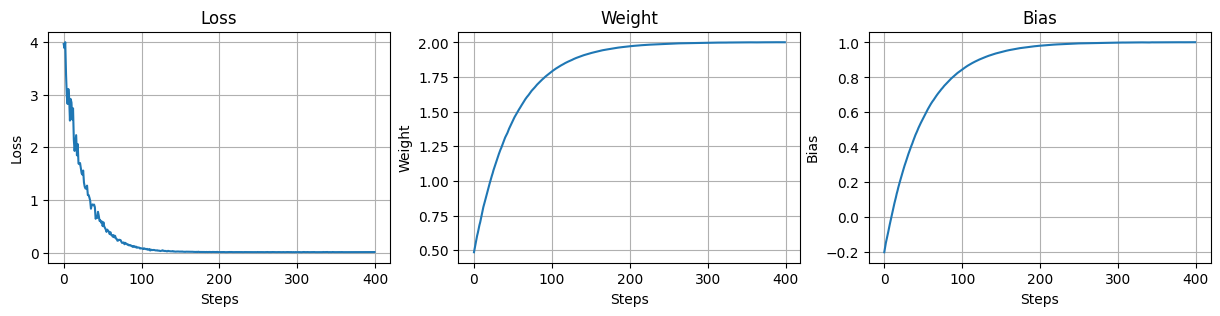
\includegraphics[width=.72\linewidth]{../../study_guide/figures/lab01/cell_025_out_00.png}\caption{Notebook output image reproduced from the saved execution.}\label{fig:lab01_cell_025_00}\end{figure}


\noindent The learned parameters are printed after training so they can be compared with the synthetic rule used to create the targets. Values near weight 2 and bias 1 indicate recovery of that rule.\par
% coverage-cell: LABS/lab01/text.ipynb cell=26 source_sha256=504b5a2f1e1e36731d75289d6b5b96ebb8e393d5f845feb3687d482dc982ff24
\begin{lstlisting}[language=Python,basicstyle=\ttfamily\scriptsize,breaklines=true,breakatwhitespace=false,columns=fullflexible,keepspaces=true,numbers=none]
# Inspecting the learned weights and biases
weights = model.linear.weight.data
biases = model.linear.bias.data

print(f'Learned weights: {weights}')
print(f'Learned biases: {biases}')
\end{lstlisting}

\label{res:lab01_cell_026}

\begin{lstlisting}[style=terminalOutput]
Learned weights: tensor([[2.0017]])
Learned biases: tensor([1.0014])
\end{lstlisting}
\chapter{Exercise 2: CIFAR-10 model training and transfer learning}
\label{ch:lab01_ex2}

The second exercise applies the same training loop to image classification and then reuses learned visual features on a related task. Its goals are to build a CIFAR-10 classifier, compare a small multilayer perceptron with a pretrained ResNet-18, and adapt the classifier head to CIFAR-100 while freezing the backbone. Inputs are RGB images with shape $[B,3,32,32]$ and integer class labels; the expected outputs are training loss curves and test accuracies. The notebook’s measured accuracies describe this specific run and hardware environment.

\section{Dataset inspection, normalization, and augmentation}

The dataset cells load batches, report their dimensions and class names, and visualize image samples. The channel statistics are calculated across the training set and used to normalize pixels. Training augmentation adds random cropping and horizontal reflection; visualization deliberately uses a separate transform so normalized values do not distort displayed colors. The saved figures below are the notebook’s original outputs.


\noindent This cell sets the environment compatibility flag before the CIFAR data loaders are constructed.\par
% coverage-cell: LABS/lab01/text.ipynb cell=28 source_sha256=0e4e0b51a1386c368b2349b7c21fe696ad5e5d397696c33f332d7573baf34fe9
\begin{lstlisting}[language=Python,basicstyle=\ttfamily\scriptsize,breaklines=true,breakatwhitespace=false,columns=fullflexible,keepspaces=true,numbers=none]
import os
dataset_dir = os.path.expanduser('~/data')
\end{lstlisting}

\label{res:lab01_cell_028}



\noindent The CIFAR-10 loader downloads or reuses the dataset, converts images to tensors, and creates shuffled training and deterministic test batches. Its output reports the image and label batch shapes and class names.\par
% coverage-cell: LABS/lab01/text.ipynb cell=29 source_sha256=675de43cd632e4073c15aa371f48a0184d83a55cb0cbeeb99410abe4ff66a14e
\begin{lstlisting}[language=Python,basicstyle=\ttfamily\scriptsize,breaklines=true,breakatwhitespace=false,columns=fullflexible,keepspaces=true,numbers=none]
# Download CIFAR-10 dataset and apply the transformations
trainset = torchvision.datasets.CIFAR10(
    root=dataset_dir, train=True, download=True, transform=transforms.ToTensor()
)

# Create a DataLoader
trainloader = torch.utils.data.DataLoader(
    trainset, batch_size=64, shuffle=True, num_workers=2
)

# Get a batch of data to verify that everything is working
# dataiter = iter(trainloader)
images, labels = next(iter(trainloader)) #dataiter.next()

print(f"Batch of images shape: {images.shape}")
print(f"Batch of labels shape: {labels.shape}")
print(f"Possible classes: {', '.join(trainset.classes)}")
\end{lstlisting}

\label{res:lab01_cell_029}

\begin{lstlisting}[style=terminalOutput]
[download progress omitted; dataset download completed, as recorded in the notebook]
/Users/nicolabeccaceci/miniconda3/lib/python3.13/site-packages/torchvision/datasets/cifar.py:83: VisibleDeprecationWarning: dtype(): align should be passed as Python or NumPy boolean but got `align=0`. Did you mean to pass a tuple to create a subarray type? (Deprecated NumPy 2.4)
  entry = pickle.load(f, encoding="latin1")
\end{lstlisting}

\begin{lstlisting}[style=terminalOutput]
Batch of images shape: torch.Size([64, 3, 32, 32])
Batch of labels shape: torch.Size([64])
Possible classes: airplane, automobile, bird, cat, deer, dog, frog, horse, ship, truck
\end{lstlisting}


\noindent The visualization displays the sampled batch as an 8-by-8 image grid. It provides a visual check that channel ordering and labels correspond to recognizable CIFAR-10 examples.\par
% coverage-cell: LABS/lab01/text.ipynb cell=31 source_sha256=cf1eac10679868f291e4e2cc5e1ab86eb510cd694e57162fef2078f40cd6543c
\begin{lstlisting}[language=Python,basicstyle=\ttfamily\scriptsize,breaklines=true,breakatwhitespace=false,columns=fullflexible,keepspaces=true,numbers=none]
import matplotlib.pyplot as plt

fig, ax = plt.subplots(8,8, figsize=(8,8))
plt.rcParams.update({'axes.titlesize': 'small'})
plt.tight_layout()
# remove vertical space
plt.subplots_adjust(hspace=0.25, wspace=0.1)

for i in range(8):
    for j in range(8):
        # note that we need to change the order of the dimensions.
        # Torch prepare the images to be (C, H, W),
        # But matplotlib expects (H, W, C)
        # (H = height of the image, W = width of the image, C = number of color channels)
        ax[i,j].imshow(images[i*8 + j].permute(1,2,0))
        ax[i,j].set_title(trainset.classes[labels[i*8 + j]])
        ax[i,j].axis('off')
\end{lstlisting}

\label{res:lab01_cell_031}
\begin{figure}[H]\centering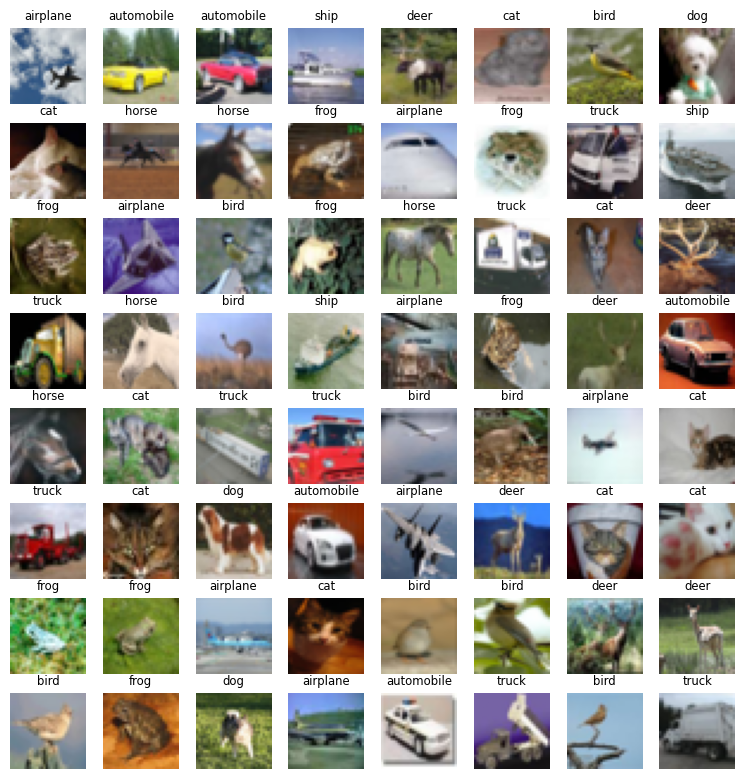
\includegraphics[width=.72\linewidth]{../../study_guide/figures/lab01/cell_031_out_00.png}\caption{Notebook output image reproduced from the saved execution.}\label{fig:lab01_cell_031_00}\end{figure}


\noindent This pass computes per-channel means and standard deviations over the training images, accounting for the channel and spatial dimensions. These statistics define a normalization transform for this dataset.\par
% coverage-cell: LABS/lab01/text.ipynb cell=33 source_sha256=297bb471a4b48d9b6cfaab89cdae45e779c5a3168dabcf5fdf452595f6e9d987
\begin{lstlisting}[language=Python,basicstyle=\ttfamily\scriptsize,breaklines=true,breakatwhitespace=false,columns=fullflexible,keepspaces=true,numbers=none]
# TODO: find the mean value and the standard deviation of the images in the dataset
# Note:
# - The images are available in trainset.data
# - Scale the images to the [0,1] range before proceeding
# - Compute a different mean and standard deviation for each color channel
scaled_data = trainset.data / 255.0
images_mean = tuple(scaled_data.mean(axis=(0, 1, 2)).tolist())
images_std = tuple(scaled_data.std(axis=(0, 1, 2)).tolist())
print(f"Mean: {images_mean}")
print(f"Std: {images_std}")
\end{lstlisting}

\label{res:lab01_cell_033}

\begin{lstlisting}[style=terminalOutput]
Mean: (0.4913996786152028, 0.4821584083946074, 0.4465309144454644)
Std: (0.24703223246328238, 0.2434851280000556, 0.26158784172796423)
\end{lstlisting}


\noindent The example transform composes random crop, horizontal flip, tensor conversion, and normalization for training-time augmentation.\par
% coverage-cell: LABS/lab01/text.ipynb cell=34 source_sha256=4b73a6c8d09235433e79696e35e6a70c2c7de8d47fde36b7464ad640b44955ae
\begin{lstlisting}[language=Python,basicstyle=\ttfamily\scriptsize,breaklines=true,breakatwhitespace=false,columns=fullflexible,keepspaces=true,numbers=none]
transform_train_example = transforms.Compose([
    transforms.RandomHorizontalFlip(),  # Randomly flip the image horizontally for the data augmentation
    transforms.RandomCrop(32, padding_mode='reflect', padding=5),  # Randomly crop the image for the data augmentation
    transforms.ToTensor(),  # Convert the image to a tensor
    transforms.Normalize(images_mean, images_std)  # Normalize the tensor
])
\end{lstlisting}

\label{res:lab01_cell_034}



\noindent This separate visualization transform omits normalization so that pixel colors remain interpretable. The resulting grid shows that random crops and flips change the displayed training examples.\par
% coverage-cell: LABS/lab01/text.ipynb cell=37 source_sha256=43c95a758d26eea8ca5a59f9fdcb592ac63fb9905f00ed88971c6d91cede720d
\begin{lstlisting}[language=Python,basicstyle=\ttfamily\scriptsize,breaklines=true,breakatwhitespace=false,columns=fullflexible,keepspaces=true,numbers=none]
viz_transform = transforms.Compose([
    transforms.RandomHorizontalFlip(),
    # note the padding_mode policy: this implies that the "missing" pixels
    # will be reflected from the border pixels
    # (more info in the documentation => https://pytorch.org/vision/main/generated/torchvision.transforms.RandomCrop.html)
    transforms.RandomCrop(32, padding_mode='reflect', padding=5)
])

im = transforms.ToPILImage()(images[10])
n_transforms = 9

fig, ax = plt.subplots(3,3, figsize=(4,4))
# TODO: Visualize the original image ,then apply different transformations to it
# Note: each time you apply the viz_transform transformation, a random transformation will be applied to the image
ax[0, 0].imshow(im)
ax[0, 0].set_title('Original', fontsize=8)
ax[0, 0].axis('off')

for i in range(1, n_transforms):
    r, c = divmod(i, 3)
    ax[r, c].imshow(viz_transform(im))
    ax[r, c].set_title(f'Aug {i}', fontsize=8)
    ax[r, c].axis('off')
plt.tight_layout()
\end{lstlisting}

\label{res:lab01_cell_037}
\begin{figure}[H]\centering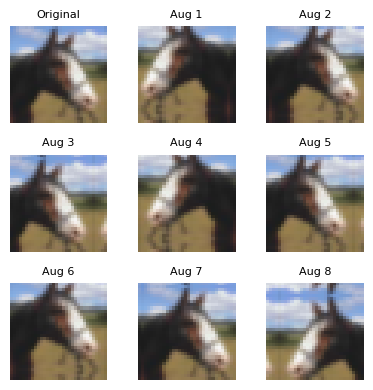
\includegraphics[width=.72\linewidth]{../../study_guide/figures/lab01/cell_037_out_00.png}\caption{Notebook output image reproduced from the saved execution.}\label{fig:lab01_cell_037_00}\end{figure}


\noindent This cell creates an initial shuffled training loader using CIFAR-10 channel statistics and augmentation. Later cells replace these dataset and loader variables before the classifier is trained, so this first loader is a preprocessing example rather than the one consumed by the subsequent training loop.\par
% coverage-cell: LABS/lab01/text.ipynb cell=39 source_sha256=688f20f9e55d7aa6ea3f955b2cdbc9582871bc4d850a7c7f2106b8d5614f4894
\begin{lstlisting}[language=Python,basicstyle=\ttfamily\scriptsize,breaklines=true,breakatwhitespace=false,columns=fullflexible,keepspaces=true,numbers=none]
# Download CIFAR-10 dataset and apply the transformations
trainset = torchvision.datasets.CIFAR10(
    root=dataset_dir, train=True, download=True, transform=transform_train_example
)

# Create a DataLoader
trainloader = torch.utils.data.DataLoader(
    trainset, batch_size=64, shuffle=True, num_workers=2
)
\end{lstlisting}

\label{res:lab01_cell_039}

\section{A multilayer perceptron baseline}

Flattening an image converts its $3\times32\times32$ pixel tensor to a vector of 3072 features. The MLP applies affine layers separated by nonlinear activations, then returns ten logits for cross-entropy classification. In this run it receives the ImageNet-normalized batches created immediately before the model, with 1024 examples per batch. The validation helper switches batch-normalization and dropout layers to evaluation behavior and disables gradient tracking. The initial accuracy gives a baseline before training; the five-epoch loss trace and second evaluation show the effect of optimization on the test set.


\noindent \texttt{SimpleNN} flattens each 3-by-32-by-32 image and applies fully connected layers with nonlinear activations before producing ten class scores. This cell defines the model class used in the baseline CIFAR-10 experiment.\par
% coverage-cell: LABS/lab01/text.ipynb cell=42 source_sha256=088fb52a832b17170dfa9e3f09d37b3b5705c8fdbf91be372cfa6cf4e9e134da
\begin{lstlisting}[language=Python,basicstyle=\ttfamily\scriptsize,breaklines=true,breakatwhitespace=false,columns=fullflexible,keepspaces=true,numbers=none]
# Define a more complex neural network model
class SimpleNN(nn.Module):
    def __init__(self):
        super(SimpleNN, self).__init__()
        # Define the linear layers for the model: each layer requires specifying the number of input and output features

        # - The first layer takes as input a flattened image (32x32x3) and should produce 512 features
        #   (i.e., it encodes the image into a 512-dimensional space)
        self.fc1 = nn.Linear(32 * 32 * 3, 512)

        # - The second layer should produce 256 features
        self.fc2 = nn.Linear(512, 256)

        # - The output layer should produce 10 features (these will be the logits)    
        self.fc3 = nn.Linear(256, 10)

    def forward(self, x):
        # Implement the forward pass

        # - first step: flatten the input (preserve the batch size, flatten the rest)
        x = x.view(x.size(0), -1)

        # - apply the first linear layer with ReLU activation
        x = F.relu(self.fc1(x))

        # - apply the second linear layer with ReLU activation
        x = F.relu(self.fc2(x))

        # - apply the output layer (no activation needed for the output layer)
        x = self.fc3(x)
        
        return x
\end{lstlisting}

\label{res:lab01_cell_042}



\noindent These transforms apply random crop and horizontal reflection to training images, then normalize both splits with ImageNet channel statistics. Although those values are motivated by the later pretrained ResNet, the notebook also uses these transforms for the MLP experiment.\par
% coverage-cell: LABS/lab01/text.ipynb cell=44 source_sha256=b76a4e65263ef4ce2d776557de3ba1b596d7cca9f7842fdde231b7afca783e6e
\begin{lstlisting}[language=Python,basicstyle=\ttfamily\scriptsize,breaklines=true,breakatwhitespace=false,columns=fullflexible,keepspaces=true,numbers=none]
# Define transformations for the training and test datasets
transform_train = transforms.Compose([
    transforms.RandomCrop(32, padding_mode='reflect', padding=4),
    transforms.RandomHorizontalFlip(),
    transforms.ToTensor(),
    transforms.Normalize(mean=[0.485, 0.456, 0.406], std=[0.229, 0.224, 0.225]), 
])

transform_test = transforms.Compose([
    transforms.ToTensor(),
    transforms.Normalize(mean=[0.485, 0.456, 0.406], std=[0.229, 0.224, 0.225]),
])
\end{lstlisting}

\label{res:lab01_cell_044}



\noindent This cell rebuilds both datasets and loaders with the ImageNet-normalized transforms and a batch size of 1024. It replaces the earlier CIFAR-statistics loader; these are the batches consumed by the MLP training and validation cells. Evaluation keeps deterministic ordering.\par
% coverage-cell: LABS/lab01/text.ipynb cell=46 source_sha256=75bc3e9b2a00a9601a0b833c0ac57ad94f82ffa0ee5931a374faf3d8da1cccee
\begin{lstlisting}[language=Python,basicstyle=\ttfamily\scriptsize,breaklines=true,breakatwhitespace=false,columns=fullflexible,keepspaces=true,numbers=none]
# Load CIFAR-10 dataset
batch_size = 1024
trainset = torchvision.datasets.CIFAR10(root=dataset_dir, train=True, download=True, transform=transform_train)
trainloader = torch.utils.data.DataLoader(trainset, batch_size=batch_size, shuffle=True)

testset = torchvision.datasets.CIFAR10(root=dataset_dir, train=False, download=True, transform=transform_test)
testloader = torch.utils.data.DataLoader(testset, batch_size=batch_size, shuffle=False)
\end{lstlisting}

\label{res:lab01_cell_046}



\noindent This cell creates the classifier, cross-entropy loss, and SGD optimizer that jointly define the CIFAR-10 training problem.\par
% coverage-cell: LABS/lab01/text.ipynb cell=47 source_sha256=2f811e62a6bcfba64f9e0ff4228affe78ebf3b531a34330253ee456b274980d8
\begin{lstlisting}[language=Python,basicstyle=\ttfamily\scriptsize,breaklines=true,breakatwhitespace=false,columns=fullflexible,keepspaces=true,numbers=none]
# Initialize the model, loss function, and optimizer
model = SimpleNN()
model = model.to(device)
criterion = nn.CrossEntropyLoss()
optimizer = optim.SGD(model.parameters(), lr=0.01, momentum=0.9)
\end{lstlisting}

\label{res:lab01_cell_047}



\noindent The validation helper switches the model to evaluation mode, disables gradient recording, accumulates correct predictions, and reports accuracy over the test loader.\par
% coverage-cell: LABS/lab01/text.ipynb cell=48 source_sha256=b4b5eb9a67a8af458b82c57fb22fe6f3965b0f7af74102677df967892a5fcfb8
\begin{lstlisting}[language=Python,basicstyle=\ttfamily\scriptsize,breaklines=true,breakatwhitespace=false,columns=fullflexible,keepspaces=true,numbers=none]
def val_model(model, testloader):
    model.eval() # NOTE: required to set the model to evaluation mode (some layers may behave differently during training and evaluation)
    correct = 0
    total = 0

    # at inference time, the model parameters are already computed and frozen, hence we have nt to recompute the new gradients
    with torch.no_grad(): # NOTE: we disable gradient tracking for validation, to save memory!
        for inputs, labels in testloader:
            inputs, labels = inputs.to(device), labels.to(device)
            outputs = model(inputs)
            _, predicted = torch.max(outputs.data, 1)
            total += labels.size(0)
            correct += (predicted == labels).sum().item()

    print(f"Accuracy of the network on the test images: {100 * correct / total:.2f}%")
\end{lstlisting}

\label{res:lab01_cell_048}



\noindent This call measures the untrained classifier’s baseline accuracy. A result near the ten-class chance level is expected before optimization.\par
% coverage-cell: LABS/lab01/text.ipynb cell=49 source_sha256=6490eaf729ef3154c05ad4b83c75ea2a625d15ed16b29d1014f3d11315e40b46
\begin{lstlisting}[language=Python,basicstyle=\ttfamily\scriptsize,breaklines=true,breakatwhitespace=false,columns=fullflexible,keepspaces=true,numbers=none]
val_model(model, testloader)
\end{lstlisting}

\label{res:lab01_cell_049}

\begin{lstlisting}[style=terminalOutput]
Accuracy of the network on the test images: 10.36%
\end{lstlisting}


\noindent The training loop processes minibatches for five epochs and records mean loss per epoch. Its output provides the learning curve data used by the following evaluation and plot.\par
% coverage-cell: LABS/lab01/text.ipynb cell=50 source_sha256=cf26e96f521e0f341a082524a20e48b05225d9ef47385a495132ce478da920fa
\begin{lstlisting}[language=Python,basicstyle=\ttfamily\scriptsize,breaklines=true,breakatwhitespace=false,columns=fullflexible,keepspaces=true,numbers=none]
# Training loop
num_epochs = 5

losses = []

model.train()
for epoch in range(num_epochs):
    running_loss = 0.0
    for inputs, labels in trainloader:
        inputs, labels = inputs.to(device), labels.to(device)

        # TODO: let's implement the training loop for the model
        # Notes:
        # - First, zero the parameter gradients
        optimizer.zero_grad()

        # - Next, get the model's predictions
        outputs = model(inputs)

        # - Compute the loss
        loss = criterion(outputs, labels)

        # - Perform backpropagation (i.e. compute all gradients)
        loss.backward()
        
        # - Finally, update the model's parameters
        optimizer.step()
        losses.append(loss.item())

        running_loss += loss.item()

    print(f"Epoch [{epoch+1}/{num_epochs}], Loss: {running_loss/len(trainloader):.4f}")
\end{lstlisting}

\label{res:lab01_cell_050}

\begin{lstlisting}[style=terminalOutput]
Epoch [1/5], Loss: 2.0972
Epoch [2/5], Loss: 1.8565
Epoch [3/5], Loss: 1.7548
Epoch [4/5], Loss: 1.6988
Epoch [5/5], Loss: 1.6535
\end{lstlisting}


\noindent Re-evaluation after training measures whether the learned parameters improved held-out classification accuracy compared with the untrained baseline.\par
% coverage-cell: LABS/lab01/text.ipynb cell=53 source_sha256=6490eaf729ef3154c05ad4b83c75ea2a625d15ed16b29d1014f3d11315e40b46
\begin{lstlisting}[language=Python,basicstyle=\ttfamily\scriptsize,breaklines=true,breakatwhitespace=false,columns=fullflexible,keepspaces=true,numbers=none]
val_model(model, testloader)
\end{lstlisting}

\label{res:lab01_cell_053}

\begin{lstlisting}[style=terminalOutput]
Accuracy of the network on the test images: 45.81%
\end{lstlisting}


\noindent This figure plots the recorded epoch losses. A declining curve supports that optimization is fitting the training data, while the curve alone does not establish generalization.\par
% coverage-cell: LABS/lab01/text.ipynb cell=55 source_sha256=7fc165ade1bbbb7165c1becf6d29ad014f09b480a6e734bdbd3a85458fb0077c
\begin{lstlisting}[language=Python,basicstyle=\ttfamily\scriptsize,breaklines=true,breakatwhitespace=false,columns=fullflexible,keepspaces=true,numbers=none]
fig, ax = plt.subplots()

ax.plot(losses)
ax.set_xlabel("Steps")
ax.set_ylabel("Loss")
\end{lstlisting}

\label{res:lab01_cell_055}
\begin{figure}[H]\centering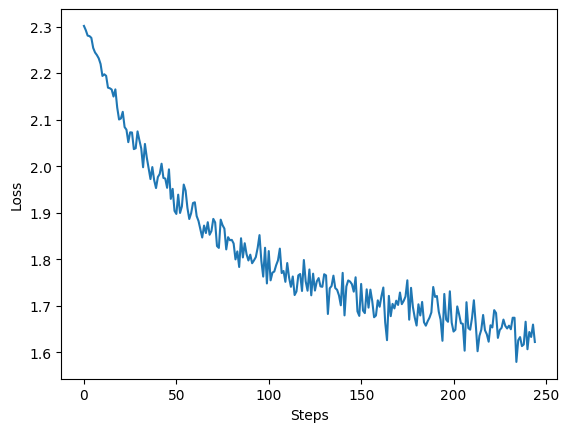
\includegraphics[width=.72\linewidth]{../../study_guide/figures/lab01/cell_055_out_01.png}\caption{Notebook output image reproduced from the saved execution.}\label{fig:lab01_cell_055_01}\end{figure}
\section{Fine-tuning a pretrained ResNet-18 on CIFAR-10}

ResNet-18 begins from ImageNet-trained convolutional features. The input pipeline uses the ImageNet channel normalization expected by those weights, and the final layer is replaced to produce ten CIFAR-10 logits. The notebook then trains and evaluates the adapted model. Its loss plot and test accuracy permit comparison with the MLP under the notebook’s settings; the observed result reflects both the pretrained representation and the chosen optimization schedule.


\noindent This cell builds the transformed CIFAR-10 loaders used for the pretrained-model experiment, keeping the ImageNet normalization required by the ResNet weights.\par
% coverage-cell: LABS/lab01/text.ipynb cell=58 source_sha256=ebc4aea12b4f05886e325e89555a0a4e1d81c9e3e93994db31475225b7744441
\begin{lstlisting}[language=Python,basicstyle=\ttfamily\scriptsize,breaklines=true,breakatwhitespace=false,columns=fullflexible,keepspaces=true,numbers=none]
# Load the CIFAR-10 dataset
trainset = torchvision.datasets.CIFAR10(root=dataset_dir, train=True, download=True, transform=transform_train)
trainloader = torch.utils.data.DataLoader(trainset, batch_size=512, shuffle=True)

testset = torchvision.datasets.CIFAR10(root=dataset_dir, train=False, download=True, transform=transform_test)
testloader = torch.utils.data.DataLoader(testset, batch_size=512, shuffle=False)
\end{lstlisting}

\label{res:lab01_cell_058}



\noindent Importing the model collection exposes torchvision’s pretrained ResNet-18 architecture for reuse.\par
% coverage-cell: LABS/lab01/text.ipynb cell=59 source_sha256=dd082972ad9c20f5d3abc7dc051e759b2d9c0eca0b90e0b95a99147132f97783
\begin{lstlisting}[language=Python,basicstyle=\ttfamily\scriptsize,breaklines=true,breakatwhitespace=false,columns=fullflexible,keepspaces=true,numbers=none]
from torchvision import models

# Load a pre-trained model (ResNet18)
model = models.resnet18(weights=None)
model.fc = nn.Linear(model.fc.in_features, 10)  # CIFAR-10 has 10 classes
model = model.to(device)
\end{lstlisting}

\label{res:lab01_cell_059}



\noindent The cross-entropy criterion compares ten class logits with integer class labels; SGD optimizes the model parameters in the following loop.\par
% coverage-cell: LABS/lab01/text.ipynb cell=60 source_sha256=8feea5ec8e7d85b7d4b641cae63efa349aac23e5cb81353818236d610f1d1e5f
\begin{lstlisting}[language=Python,basicstyle=\ttfamily\scriptsize,breaklines=true,breakatwhitespace=false,columns=fullflexible,keepspaces=true,numbers=none]
# Define loss function and optimizer
criterion = nn.CrossEntropyLoss()
optimizer = optim.SGD(model.parameters(), lr=0.01, momentum=0.9, weight_decay=5e-4)
\end{lstlisting}

\label{res:lab01_cell_060}



\noindent The loop fine-tunes the selected ResNet on CIFAR-10 for five epochs and reports mean batch loss for each epoch.\par
% coverage-cell: LABS/lab01/text.ipynb cell=61 source_sha256=0bf241c708c09ccb6ea3c708cea1bf01c98b4aa643b5b68283c0a78086548bf1
\begin{lstlisting}[language=Python,basicstyle=\ttfamily\scriptsize,breaklines=true,breakatwhitespace=false,columns=fullflexible,keepspaces=true,numbers=none]
# Training loop
num_epochs = 5

losses = []

model.train()
for epoch in range(num_epochs):
    running_loss = 0.0
    for inputs, labels in trainloader:
        inputs, labels = inputs.to(device), labels.to(device)

        # Zero the parameter gradients
        optimizer.zero_grad()

        # Forward pass
        outputs = model(inputs)
        loss = criterion(outputs, labels)

        # Backward pass and optimization
        loss.backward()
        optimizer.step()

        losses.append(loss.item())

        running_loss += loss.item()

    print(f"Epoch [{epoch+1}/{num_epochs}], Loss: {running_loss/len(trainloader):.4f}")
\end{lstlisting}

\label{res:lab01_cell_061}

\begin{lstlisting}[style=terminalOutput]
Epoch [1/5], Loss: 1.7461
Epoch [2/5], Loss: 1.4103
Epoch [3/5], Loss: 1.2676
Epoch [4/5], Loss: 1.1643
Epoch [5/5], Loss: 1.0799
\end{lstlisting}


\noindent This call evaluates the fine-tuned ResNet on CIFAR-10 test images and prints its held-out accuracy.\par
% coverage-cell: LABS/lab01/text.ipynb cell=62 source_sha256=f9bc453e919fd41802a8a7deb1213a6362a9007c26a1452b25dca62702f43e36
\begin{lstlisting}[language=Python,basicstyle=\ttfamily\scriptsize,breaklines=true,breakatwhitespace=false,columns=fullflexible,keepspaces=true,numbers=none]
# Validate the model
val_model(model, testloader)
\end{lstlisting}

\label{res:lab01_cell_062}

\begin{lstlisting}[style=terminalOutput]
Accuracy of the network on the test images: 63.56%
\end{lstlisting}


\noindent The plot summarizes the ResNet training losses across epochs, allowing comparison with the earlier small network.\par
% coverage-cell: LABS/lab01/text.ipynb cell=63 source_sha256=7fc165ade1bbbb7165c1becf6d29ad014f09b480a6e734bdbd3a85458fb0077c
\begin{lstlisting}[language=Python,basicstyle=\ttfamily\scriptsize,breaklines=true,breakatwhitespace=false,columns=fullflexible,keepspaces=true,numbers=none]
fig, ax = plt.subplots()

ax.plot(losses)
ax.set_xlabel("Steps")
ax.set_ylabel("Loss")
\end{lstlisting}

\label{res:lab01_cell_063}
\begin{figure}[H]\centering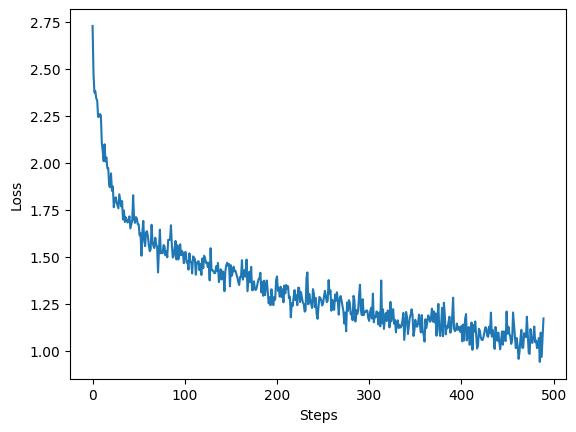
\includegraphics[width=.72\linewidth]{../../study_guide/figures/lab01/cell_063_out_01.png}\caption{Notebook output image reproduced from the saved execution.}\label{fig:lab01_cell_063_01}\end{figure}


\noindent The pretrained ResNet-18 weights are loaded, its 1000-class final layer is replaced with a ten-class classifier, and the model is moved to the selected device. The notebook output confirms the weight checkpoint was obtained.\par
% coverage-cell: LABS/lab01/text.ipynb cell=65 source_sha256=f1cdc4bb7d065287b919e103c3f8532633c931912bb5dc7a75feb7a18c9cebce
\begin{lstlisting}[language=Python,basicstyle=\ttfamily\scriptsize,breaklines=true,breakatwhitespace=false,columns=fullflexible,keepspaces=true,numbers=none]
# Load a pre-trained model (ResNet18)
pretrained_model = models.resnet18(weights='DEFAULT')

# The model has a fully connected layer at the end (called `fc`) that needs to be replaced with a new one of the appropriate size
pretrained_model.fc = nn.Linear(pretrained_model.fc.in_features, 10)

# To get the number of input features for the new layer, you can access the in_features attribute of the original fc layer
pretrained_model = pretrained_model.to(device) # move the model (all layers, even new ones) to the device
\end{lstlisting}

\label{res:lab01_cell_065}

\begin{lstlisting}[style=terminalOutput]
Downloading: "https://download.pytorch.org/models/resnet18-f37072fd.pth" to /Users/nicolabeccaceci/.cache/torch/hub/checkpoints/resnet18-f37072fd.pth
\end{lstlisting}

\begin{lstlisting}[style=terminalOutput]
[download progress omitted; dataset download completed, as recorded in the notebook]
\end{lstlisting}


\noindent This cell configures cross-entropy for the CIFAR-10 labels and an optimizer for the parameters that remain trainable in the pretrained model.\par
% coverage-cell: LABS/lab01/text.ipynb cell=66 source_sha256=921e8d78d510eb5590e72bc739c6077cc5c11f5cba133bb9ee9a80f59f669bbc
\begin{lstlisting}[language=Python,basicstyle=\ttfamily\scriptsize,breaklines=true,breakatwhitespace=false,columns=fullflexible,keepspaces=true,numbers=none]
criterion = nn.CrossEntropyLoss()
optimizer = optim.SGD(pretrained_model.parameters(), lr=0.01, momentum=0.9, weight_decay=5e-4)
\end{lstlisting}

\label{res:lab01_cell_066}



\noindent This loop updates the pretrained model on CIFAR-10 for five epochs and records the resulting loss trajectory.\par
% coverage-cell: LABS/lab01/text.ipynb cell=67 source_sha256=faf1160be06dc93d669e167d30018af9ab1f13dfbaa08774ca6d0b7a4c35cfd2
\begin{lstlisting}[language=Python,basicstyle=\ttfamily\scriptsize,breaklines=true,breakatwhitespace=false,columns=fullflexible,keepspaces=true,numbers=none]
# Training loop
num_epochs = 5

losses = []

model.train()
for epoch in range(num_epochs):
    running_loss = 0.0
    for inputs, labels in trainloader:
        inputs, labels = inputs.to(device), labels.to(device)

        # Zero the parameter gradients
        optimizer.zero_grad()

        # Forward pass
        outputs = pretrained_model(inputs)
        loss = criterion(outputs, labels)

        # Backward pass and optimization
        loss.backward()
        optimizer.step()

        losses.append(loss.item())

        running_loss += loss.item()

    print(f"Epoch [{epoch+1}/{num_epochs}], Loss: {running_loss/len(trainloader):.4f}")
\end{lstlisting}

\label{res:lab01_cell_067}

\begin{lstlisting}[style=terminalOutput]
Epoch [1/5], Loss: 1.1265
Epoch [2/5], Loss: 0.6969
Epoch [3/5], Loss: 0.5946
Epoch [4/5], Loss: 0.5338
Epoch [5/5], Loss: 0.4921
\end{lstlisting}


\noindent The evaluation call reports the test accuracy obtained by the adapted pretrained model.\par
% coverage-cell: LABS/lab01/text.ipynb cell=68 source_sha256=fcbfe787f2ccce921b6755974b835a4f234e2d35827aad99926dadfe0e020ee9
\begin{lstlisting}[language=Python,basicstyle=\ttfamily\scriptsize,breaklines=true,breakatwhitespace=false,columns=fullflexible,keepspaces=true,numbers=none]
val_model(pretrained_model, testloader)
\end{lstlisting}

\label{res:lab01_cell_068}

\begin{lstlisting}[style=terminalOutput]
Accuracy of the network on the test images: 81.66%
\end{lstlisting}


\noindent This plot shows the epoch losses for the adapted ResNet and makes its optimization behavior visible.\par
% coverage-cell: LABS/lab01/text.ipynb cell=69 source_sha256=7fc165ade1bbbb7165c1becf6d29ad014f09b480a6e734bdbd3a85458fb0077c
\begin{lstlisting}[language=Python,basicstyle=\ttfamily\scriptsize,breaklines=true,breakatwhitespace=false,columns=fullflexible,keepspaces=true,numbers=none]
fig, ax = plt.subplots()

ax.plot(losses)
ax.set_xlabel("Steps")
ax.set_ylabel("Loss")
\end{lstlisting}

\label{res:lab01_cell_069}
\begin{figure}[H]\centering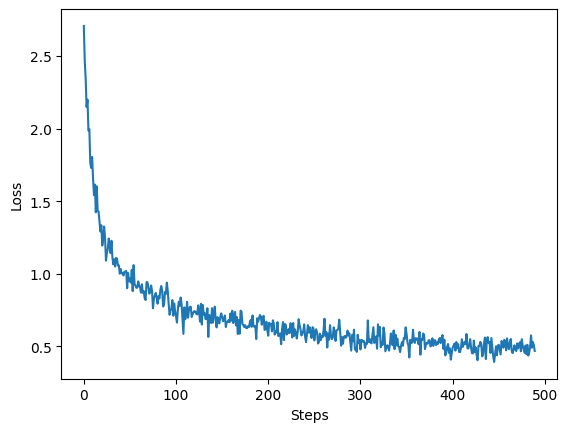
\includegraphics[width=.72\linewidth]{../../study_guide/figures/lab01/cell_069_out_01.png}\caption{Notebook output image reproduced from the saved execution.}\label{fig:lab01_cell_069_01}\end{figure}
\section{Adapting the classifier head to CIFAR-100}

CIFAR-100 introduces a new label space with one hundred classes. Replacing the final layer changes the output dimension; freezing all other parameters restricts learning to the new head. The optimizer receives only those trainable parameters. After one epoch, the notebook reports loss and test accuracy and plots the loss. Because the backbone was originally trained on ImageNet and the head was adapted for only one epoch, this result is an initial transfer-learning measurement rather than evidence of a fully optimized CIFAR-100 classifier.

\noindent The CIFAR-100 loaders apply the same channel normalization and batch policy to the new 100-class dataset.\par
% coverage-cell: LABS/lab01/text.ipynb cell=71 source_sha256=d5e3626fea02ea4e2596096eaa9325e83214d873f5ecf9177e668cbfad044f08
\begin{lstlisting}[language=Python,basicstyle=\ttfamily\scriptsize,breaklines=true,breakatwhitespace=false,columns=fullflexible,keepspaces=true,numbers=none]
# Load the CIFAR-100 dataset
trainset_cifar100 = torchvision.datasets.CIFAR100(root=dataset_dir, train=True, download=True, transform=transform_train)
trainloader_cifar100 = torch.utils.data.DataLoader(trainset_cifar100, batch_size=100, shuffle=True)

testset_cifar100 = torchvision.datasets.CIFAR100(root=dataset_dir, train=False, download=True, transform=transform_test)
testloader_cifar100 = torch.utils.data.DataLoader(testset_cifar100, batch_size=100, shuffle=False)
\end{lstlisting}

\label{res:lab01_cell_071}

\begin{lstlisting}[style=terminalOutput]
[download progress omitted; dataset download completed, as recorded in the notebook]
\end{lstlisting}


\noindent The assignment \texttt{model = pretrained\_model} creates another name for the same module; it does not copy the network. Replacing its final fully connected layer therefore changes that module from ten outputs to one hundred, matching the CIFAR-100 label space.\par
% coverage-cell: LABS/lab01/text.ipynb cell=72 source_sha256=1e07695d8099431d54d2e268b480a110ee7a3fb801094462c03230be4dd1a640
\begin{lstlisting}[language=Python,basicstyle=\ttfamily\scriptsize,breaklines=true,breakatwhitespace=false,columns=fullflexible,keepspaces=true,numbers=none]
# Modify the classification head for CIFAR-100 (100 classes)

model = pretrained_model
model.fc = nn.Linear(model.fc.in_features, 100)
model = model.to(device)
\end{lstlisting}

\label{res:lab01_cell_072}



\noindent The parameter loop freezes the pretrained backbone and re-enables gradients only for the new classifier head, so feature extraction weights remain fixed during adaptation.\par
% coverage-cell: LABS/lab01/text.ipynb cell=74 source_sha256=84fa2c1e1bf7f2b229957ebceb8ac908ae331119b6dac4bf284abff041fb7a61
\begin{lstlisting}[language=Python,basicstyle=\ttfamily\scriptsize,breaklines=true,breakatwhitespace=false,columns=fullflexible,keepspaces=true,numbers=none]
# Freeze all layers except the classification head
for param in model.parameters():
    param.requires_grad = False

# Unfreeze the classification head
for param in model.fc.parameters():
    param.requires_grad = True
\end{lstlisting}

\label{res:lab01_cell_074}



\noindent SGD is restricted to the trainable classifier parameters; the optimizer therefore cannot change the frozen backbone.\par
% coverage-cell: LABS/lab01/text.ipynb cell=75 source_sha256=fc90f79d1b4f8afacde529d702cb105e327917ce5eed88fdc85d1f1342b4627c
\begin{lstlisting}[language=Python,basicstyle=\ttfamily\scriptsize,breaklines=true,breakatwhitespace=false,columns=fullflexible,keepspaces=true,numbers=none]
optimizer = optim.SGD(model.fc.parameters(), lr=0.01, momentum=0.9, weight_decay=5e-4)
\end{lstlisting}

\label{res:lab01_cell_075}



\noindent This single-epoch loop trains the new classifier on CIFAR-100 and reports the mean training loss.\par
% coverage-cell: LABS/lab01/text.ipynb cell=76 source_sha256=a27a22425e055e83b8bc4509106b750808100faf7356677db9c0d6fc44186993
\begin{lstlisting}[language=Python,basicstyle=\ttfamily\scriptsize,breaklines=true,breakatwhitespace=false,columns=fullflexible,keepspaces=true,numbers=none]
num_epochs = 1

losses = []

model.train()
for epoch in range(num_epochs):
    running_loss = 0.0
    for inputs, labels in trainloader_cifar100:
        inputs, labels = inputs.to(device), labels.to(device)

        # Zero the parameter gradients
        optimizer.zero_grad()

        # Forward pass
        outputs = model(inputs)
        loss = criterion(outputs, labels)

        # Backward pass and optimization
        loss.backward()
        optimizer.step()

        losses.append(loss.item())

        running_loss += loss.item()

    print(f"Epoch [{epoch+1}/{num_epochs}], Loss: {running_loss/len(trainloader_cifar100):.4f}")
\end{lstlisting}

\label{res:lab01_cell_076}

\begin{lstlisting}[style=terminalOutput]
Epoch [1/1], Loss: 3.2483
\end{lstlisting}


\noindent The model is evaluated on the CIFAR-100 test split, reporting accuracy after one epoch of head-only adaptation.\par
% coverage-cell: LABS/lab01/text.ipynb cell=77 source_sha256=c6d0aa877bafefa22cc99104163df8b965e0fe2b03462633db77e9f00a7e5e01
\begin{lstlisting}[language=Python,basicstyle=\ttfamily\scriptsize,breaklines=true,breakatwhitespace=false,columns=fullflexible,keepspaces=true,numbers=none]
val_model(model, testloader_cifar100)
\end{lstlisting}

\label{res:lab01_cell_077}

\begin{lstlisting}[style=terminalOutput]
Accuracy of the network on the test images: 28.45%
\end{lstlisting}


\noindent The plot presents the recorded CIFAR-100 training loss for the adaptation run.\par
% coverage-cell: LABS/lab01/text.ipynb cell=78 source_sha256=7fc165ade1bbbb7165c1becf6d29ad014f09b480a6e734bdbd3a85458fb0077c
\begin{lstlisting}[language=Python,basicstyle=\ttfamily\scriptsize,breaklines=true,breakatwhitespace=false,columns=fullflexible,keepspaces=true,numbers=none]
fig, ax = plt.subplots()

ax.plot(losses)
ax.set_xlabel("Steps")
ax.set_ylabel("Loss")
\end{lstlisting}

\label{res:lab01_cell_078}
\begin{figure}[H]\centering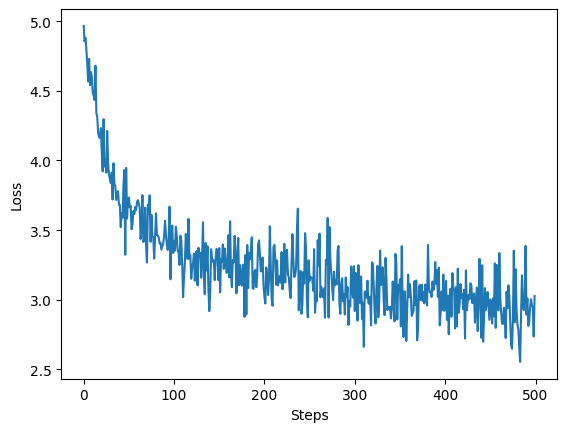
\includegraphics[width=.72\linewidth]{../../study_guide/figures/lab01/cell_078_out_01.png}\caption{Notebook output image reproduced from the saved execution.}\label{fig:lab01_cell_078_01}\end{figure}


\chapter{Exercise 3: PyTorch computational graph and backpropagation}
\label{ch:lab01_ex3}

This exercise isolates the chain rule on a small scalar computation so that the gradient path remains visible. The objective is to compute the partial derivatives of $\mathcal{L}=(\theta_1\theta_2x-y)^2$ with respect to both parameters and verify the analytical values using PyTorch autograd. The inputs $x$, $y$, $\theta_1$, and $\theta_2$ are scalars; the expected result is a graph of intermediate operations and matching gradients.

\section{Forward graph, local derivatives, and gradient accumulation}

The graph cells represent the forward computation and its intermediate values. The first graph is a separate scalar illustration with variables $a$, $b$, and $c$; it shows how repeated use of a variable creates multiple paths through the graph. The following graph defines the assigned loss with $\theta_1=2$, $\theta_2=3$, $x=1$, and target $y=3$. The prediction is $6$, so the residual is $3$ and the loss is $9$. The chain rule gives $\partial\mathcal{L}/\partial\theta_1=18$ and $\partial\mathcal{L}/\partial\theta_2=12$, which are the values printed after the backward pass.


\noindent This cell constructs a Graphviz representation of the scalar computation used in the exercise. The graph makes the dependency order explicit before gradients are calculated.\par
% coverage-cell: LABS/lab01/text.ipynb cell=80 source_sha256=86cc2e65b59c73f4d1b5202bd5ddae9dbaf317f5901dc853c823de57b8bb4661
\begin{lstlisting}[language=Python,basicstyle=\ttfamily\scriptsize,breaklines=true,breakatwhitespace=false,columns=fullflexible,keepspaces=true,numbers=none]
import torch
from torchviz import make_dot

# Define tensors with requires_grad=True to track operations
a = torch.tensor(2.0, requires_grad=True)
b = torch.tensor(3.0, requires_grad=True)
c = torch.tensor(4.0, requires_grad=True)

# Define a function involving these tensors
y = (a*b*c+c)*c + b

# Visualize the computational graph
make_dot(y, params={"a": a, "b": b, "c": c})
\end{lstlisting}

\label{res:lab01_cell_080}
\begin{figure}[H]\centering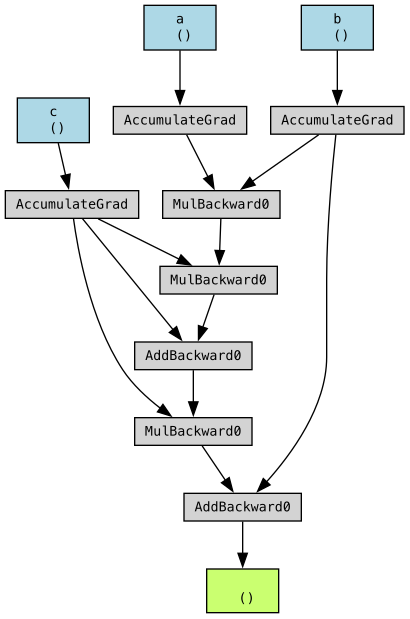
\includegraphics[width=.72\linewidth]{../../study_guide/figures/lab01/cell_080_out_00.png}\caption{Notebook output image reproduced from the saved execution.}\label{fig:lab01_cell_080_00}\end{figure}


\noindent The second graph construction expands the example into its intermediate operations, showing where each local derivative enters the chain rule.\par
% coverage-cell: LABS/lab01/text.ipynb cell=83 source_sha256=5da920e0ee397aefa82553a6558b14f1180cfaaec804455f607e5c83ce38e3b1
\begin{lstlisting}[language=Python,basicstyle=\ttfamily\scriptsize,breaklines=true,breakatwhitespace=false,columns=fullflexible,keepspaces=true,numbers=none]
import torch
from torchviz import make_dot

# Define the tensors and compute the loss
# Define theta1, theta2, x, and y as tensors, then compute the loss
# Notes:
# - set theta1 = 2.0, theta2 = 3.0, x = 1.0, y = 3.0
# - the loss is defined as (theta1 * theta2 * x - y)^2
# - all the tensors should be specified to require gradients
theta1 = torch.tensor(2.0, requires_grad=True)
theta2 = torch.tensor(3.0, requires_grad=True)
x = torch.tensor(1.0, requires_grad=True)
y = torch.tensor(3.0, requires_grad=True)

loss = (theta1 * theta2 * x - y)**2

# Visualize the computational graph
make_dot(loss, params={'theta1': theta1, 'theta2': theta2, 'x': x, 'y': y})
\end{lstlisting}

\label{res:lab01_cell_083}
\begin{figure}[H]\centering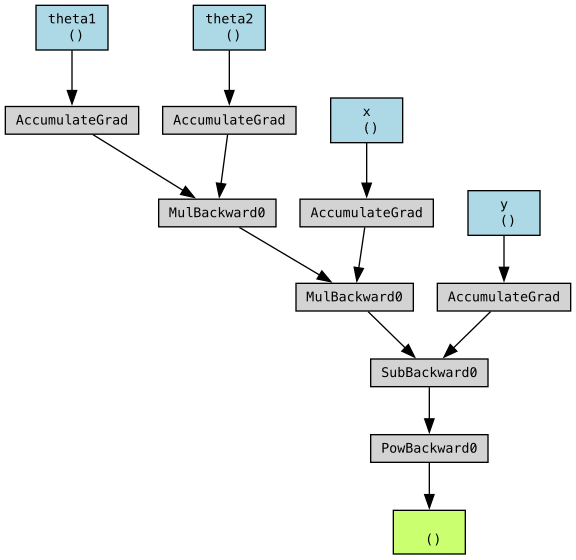
\includegraphics[width=.72\linewidth]{../../study_guide/figures/lab01/cell_083_out_00.png}\caption{Notebook output image reproduced from the saved execution.}\label{fig:lab01_cell_083_00}\end{figure}


\noindent Calling \texttt{backward()} propagates the derivative from the scalar loss to both parameters. The printed gradients are the numerical result for the values defined in the preceding graph cells.\par
% coverage-cell: LABS/lab01/text.ipynb cell=84 source_sha256=574bc7bf6dacba873a68895ae31f238bc168faab731bc2e8097d229cb89a48b2
\begin{lstlisting}[language=Python,basicstyle=\ttfamily\scriptsize,breaklines=true,breakatwhitespace=false,columns=fullflexible,keepspaces=true,numbers=none]
# Perform backpropagation to compute gradients
loss.backward()

print("Loss:", loss.item())
print("Gradients:")
print("dL/d(theta1):", theta1.grad)
print("dL/d(theta2):", theta2.grad)
\end{lstlisting}

\label{res:lab01_cell_084}

\begin{lstlisting}[style=terminalOutput]
Loss: 9.0
Gradients:
dL/d(theta1): tensor(18.)
dL/d(theta2): tensor(12.)
\end{lstlisting}
\section{What the three exercises establish}

Together, the exercises connect the main elements of a learning system: tensors carry data, modules define differentiable computations, losses measure task error, and optimizers update parameters using gradients. The image experiments add batching, normalization, evaluation mode, and transfer learning; the scalar graph makes the chain rule explicit. The results also show why training loss and test accuracy answer different questions: a decreasing objective records optimization progress, while test accuracy measures performance on unseen examples under a specified evaluation procedure.

\end{document}
